\begin{anexosenv}

\partanexos

\chapter{Primeiro Anexo}
\label{chap:anexoA}

Texto do primeiro anexo.

\begin{figure}[!htb]
	\centering
    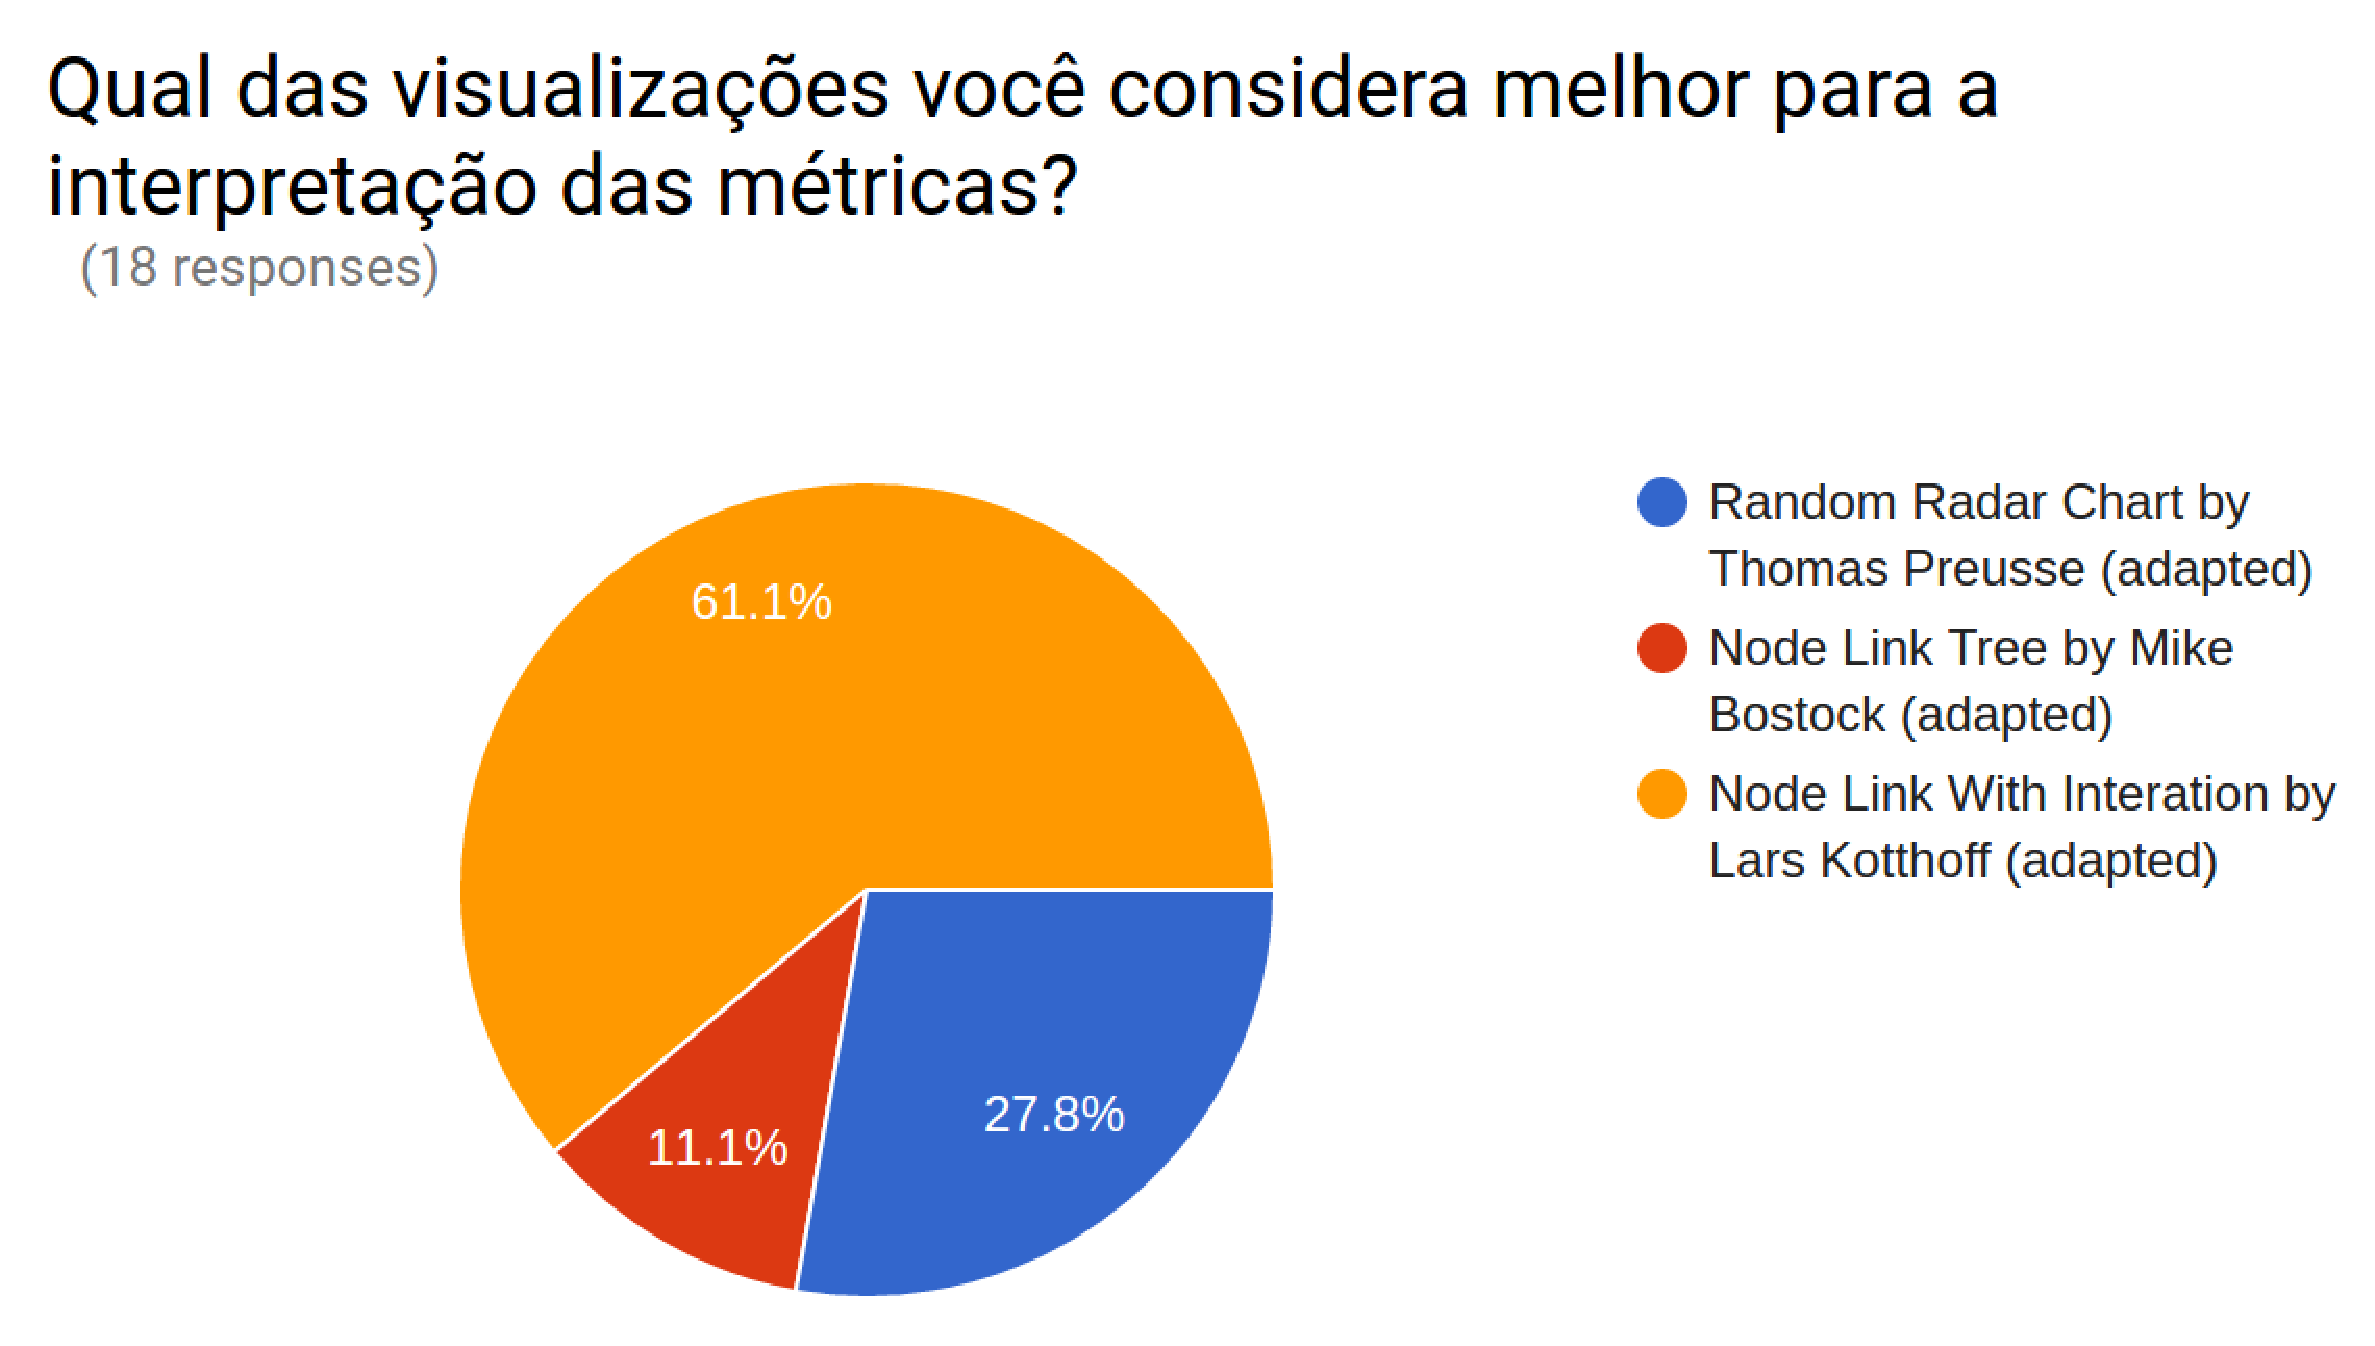
\includegraphics[keepaspectratio=true,scale=0.35]
    {figuras/res1.eps}
  \caption{Respostas para qual visualização foi considerada de melhor
  interpretação}
  \label{fig:res1}
\end{figure}

\begin{figure}[!htb]
	\centering
    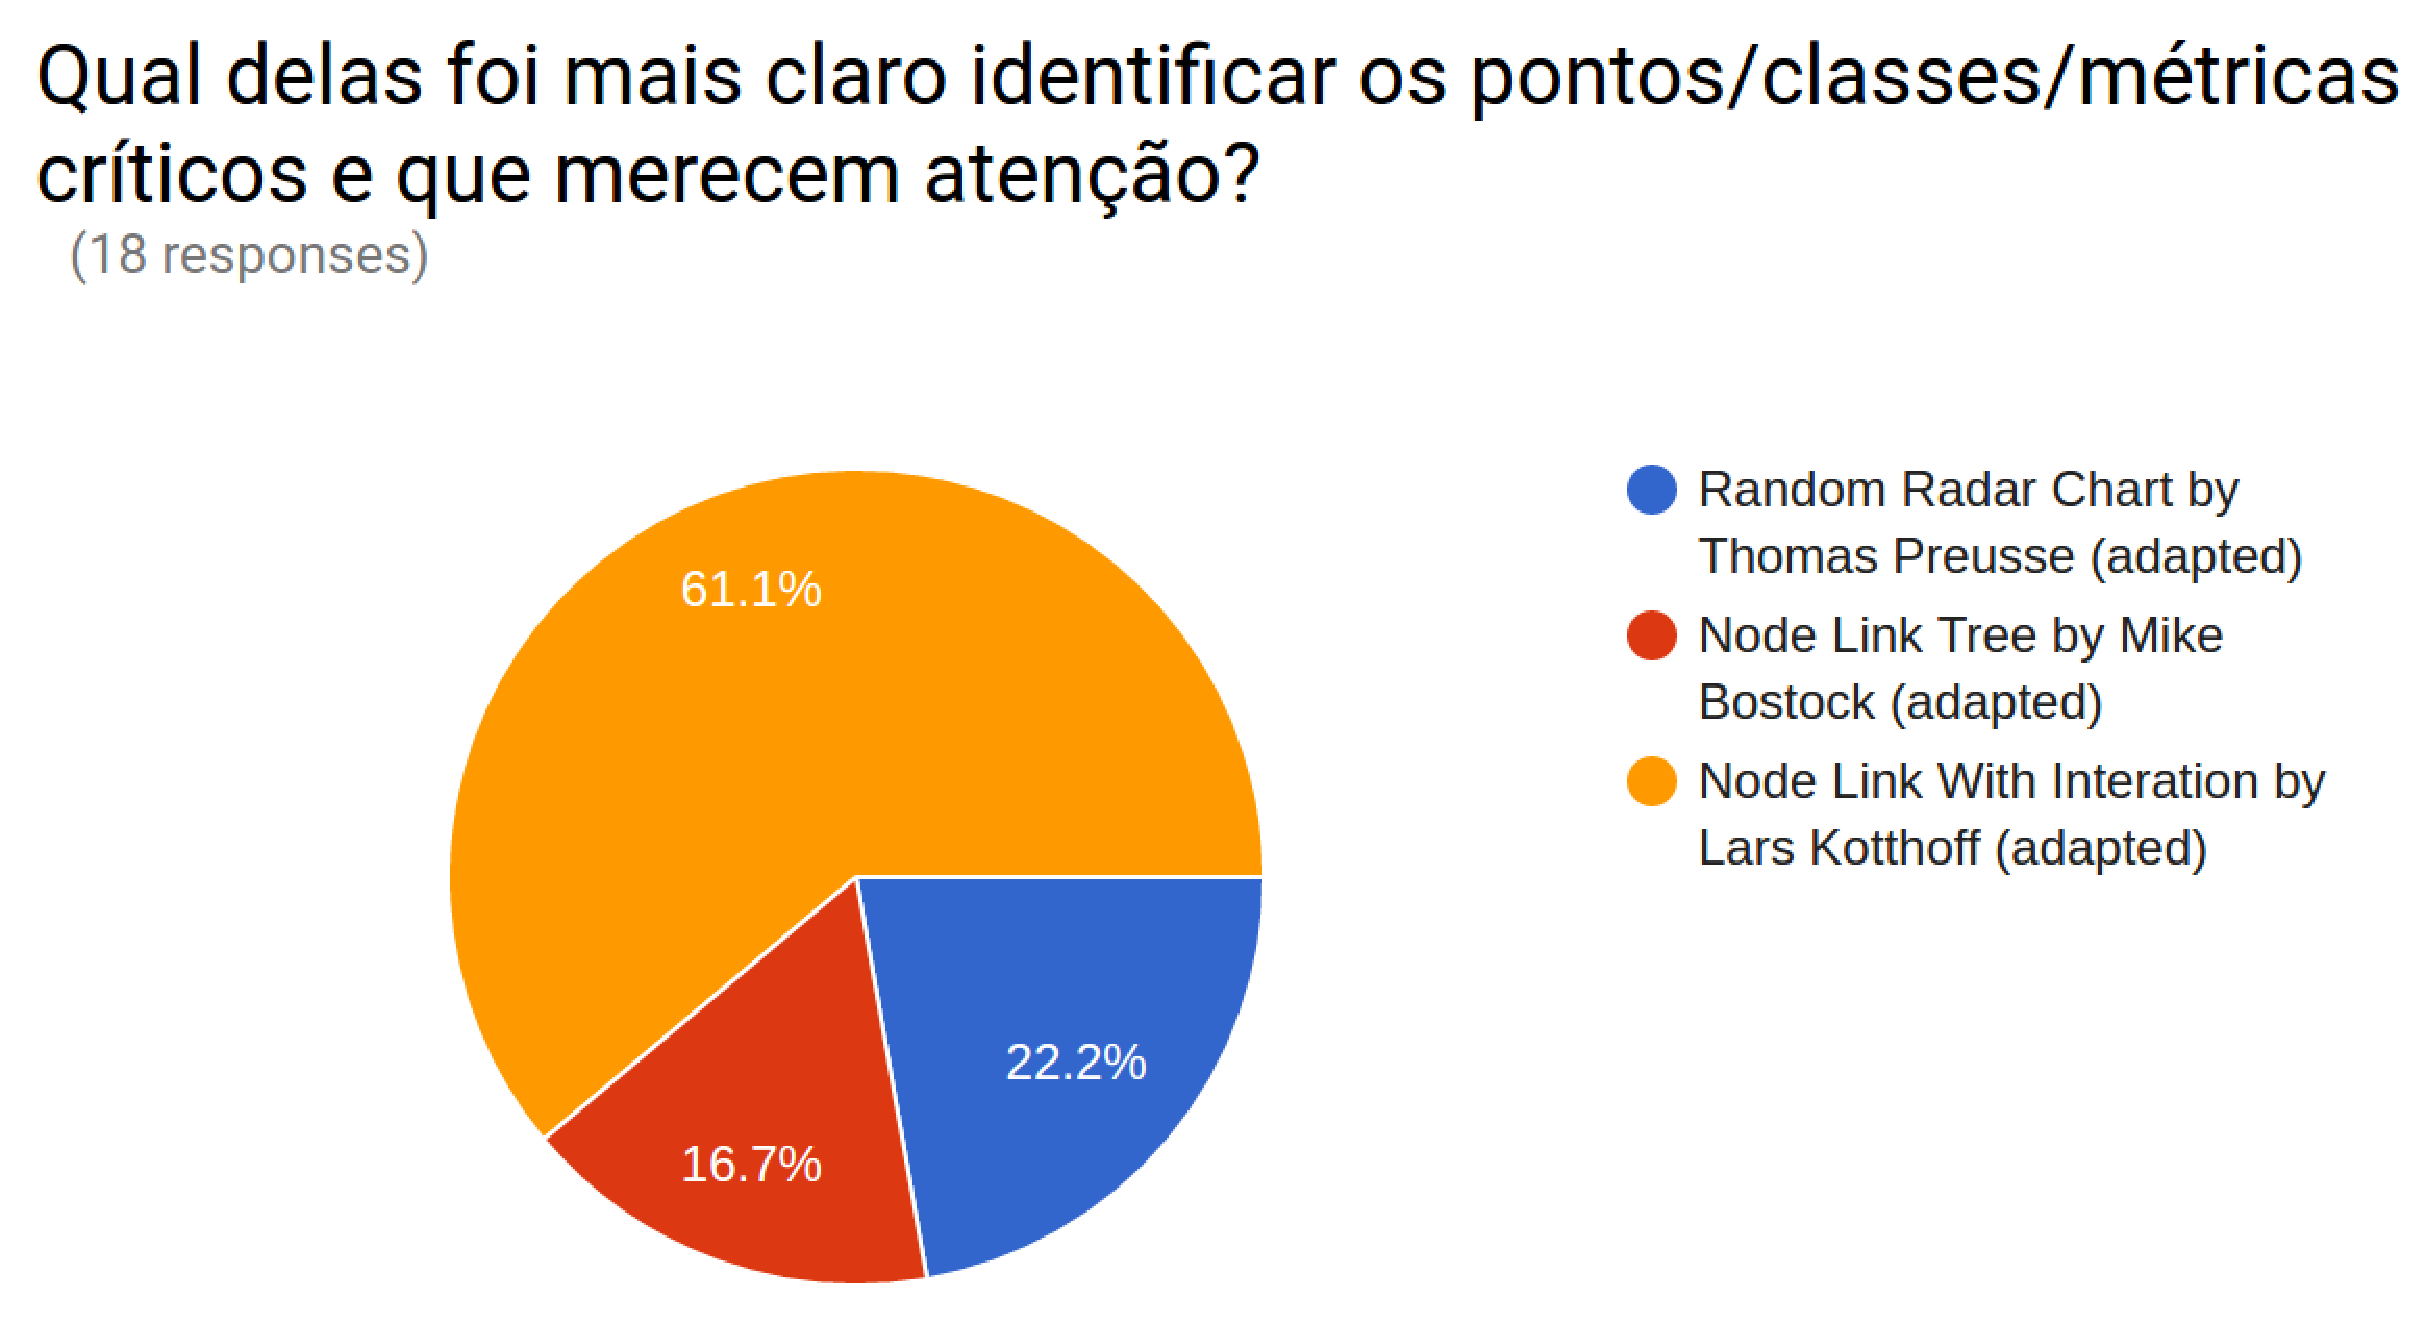
\includegraphics[keepaspectratio=true,scale=0.35]
    {figuras/res2.eps}
  \caption{Respostas para qual visualização possuia maior clareza na
  identificação dos pontos críticos}
  \label{fig:res1}
\end{figure}

Comentários, críticas e sugestões (6 respostas). Todas as respostas foram
anônimas:

\textit{"Se o método de Node With Interations, do Lars Kotthoff, começasse com
alguns nós expandidos, ele seria o melhor (na minha opinião) de longe. Como
isso não está ocorrendo, ele ainda continua melhor (na minha opinião), mas os
outros dois são mais claros para se ver o resultado final a respeito das
métricas."}

\textit{"O primeiro eu não entendi como funciona, se entendesse deve ser legal. O
segundo me deu dor de cabeça só de abrir a imagem e é ruim ficar virando a
cabeça e espremendo os olhos pra enxergar (tenho miopia)  O terceiro é legal
porque mostra tudo separadinho mas é um saco ter que clicar mil vezes pra ver
tudo."}

\textit{"Poderia colocar uma opção de visualização: Node Link With Interation
by Lars Kotthoff de vizsualizar tudo de uma vez, um expand all.}

\textit{"Para a forma de visualização do Node Link With Interation by Lars
Kotthoff (adapted) seria interessante ter um aspecto de botão para a pessoa
saber que o elemento é para ser clicado."}

\textit{"A nível de entendimento e clareza a visualização em Node Link With
Interation é a melhor, no entanto a que se apresenta de forma mais bonita é a
Node Link Tree, embora não seja tão intuitiva quanto a anterior. Além disso, a
No Link With Interation parece ter demonstrado ter capturado melhor as
necessidades, conforme a leitura das métricas, na medida em que visualmente
aponta mais valores em VERMELHO que a opção Node Link Tree. A Random Radar
Chart não evidencia valores. Não há uma escala, o que dificulta
o entendimento da gravidade da situação de uma determinada métrica."}

\textit{"Node Link Tree by Mike Bostock é a melhor, mas para ser o mais claro é
preciso trabalhar melhor com as cores usando os valores agregados de métricas.
Coloque cores em todos os nós do grafo de acordo com o grade."}


\chapter{Segundo Anexo}

Texto do segundo anexo.

\end{anexosenv}
